%%% Local Variables:
%%% mode: latex
%%% TeX-master: null
%%% End:

\documentclass[master]{sduthesis}
% \documentclass[%
%   master|doctor,              % mandatory option
%   xetex|pdftex|dvips|dvipdfm, % optional
%   secret,                     % optional
%   equival,engineer            % optional
%   openany|openright,          % optional
%   arial,arialtoc,arialtitle   % optional
% ]{sduthesis}

% 用到的宏包都统一放到了sdutils中,
% 可以根据自己的实际在sdutils.sty中添加或者删除。
\usepackage{sdutils}

\begin{document}
% 图片目录
\graphicspath{{fig/}}


%%% 1.前序部分
\frontmatter
% 封面,博士有英文封面
%%% Local Variables:
%%% mode: latex
%%% TeX-master: "../main.tex"
%%% End:

\catalognumber{TP393}
\schoolnumber{10422}
\secretlevel{内部} \secretyear{5}% 必须打开secret选项才有效
\studentnumber{201113XXX}

\ctitle{\sduthesis 示例文档}
\etitle{AN EXAMPLE DOCUMENT OF \sduthesis}
\cauthor{王克瑞}
\cdepartment{计算机科学与技术学院}
\cmajor{计算机应用技术}
\csupervisor{某某某\hspace{1em}教授}
\ccosupervisor{某某\hspace{1em}副教授}
% 日期自动生成,如果你要自己写就改这个cdate
\cdate{\the\year 年\the\month 月\the\day 日}

% 以下是博士的英文封面项。如果你是硕士,never mind
\eauthor{Wang Kerui}
\esupervisor{Prof.\:\ Mou Moumou}
\ecosupervisor{Prof.\:\ Mou Mou}
\eaddress{Shandong University, Jinan, Shandong, P.R.China}
\edate{April 30, 2014}

\makecover

% 原创性声明和关于学位论文使用授权的声明
%%%
%%% Originality Statement & Authorization Statement.
%%%
%%% File:   data/statement.tex
%%% Date:   4/23/2014
%%% Author: wkr@wangkerui.com
%%%

\originalitytitle{原\quad 创\quad 性\quad 声\quad 明}
\originalitycontent{本人郑重声明:所呈交的学位论文,是本人在导师的指导下,独立进行研究所取得的成果。除文中已经注明引用的内容外,本论文不包含任何其他个人或集体已经发表或撰写过的科研成果。对本文的研究作出重要贡献的个人和集体,均已在文中以明确方式标明。本声明的法律责任由本人承担。}

\authorizationtitle{关于学位论文使用授权的声明}
\authorizationcontent{本人同意学校保留或向国家有关部门或机构送交论文的印刷件和电子版,允许论文被查阅和借阅;本人授权山东大学可以将本学位论文的全部或部分内容编入有关数据库进行检索,可以采用影印、缩印或其他复制手段保存论文和汇编本学位论文。}
\authorizationaddon{(保密论文在解密后应遵守此规定)}

%%%
%%% End of file.
%%%

\makestatement

% 目录
\begin{contents}
\tableofcontents%  中文目录
\tableofecontents% 英文目录
\end{contents}

% 摘要(包括中文摘要和英文摘要)
%%%
%%% File:       abstract.tex
%%% TeX-Master: ../main.tex
%%% Desc:       Including Chinese & English Abstract.
%%%

% 中文摘要
\chapter{摘\hspace{1em}要}
\echapter{Chinese Abstract}
这里写摘要。请注意:务必先浏览 sduthesis.pdf 的前 4 章,然后再结合本示例文档写作论文。

本示例文档主要示例如何使用本模板排版,基本上和标准类模板没差。包括,章节标题,英文目录,公式、算法,插图、表格,定义、定理和证明环境等。

填充废话。

豫章故郡,洪都新府。星分翼轸(zhěn),地接衡庐。襟三江而带五湖,控蛮荆而引瓯(ōu)越。物华天宝,龙光射牛斗之墟;人杰地灵,徐孺下陈蕃(fān)之榻(tà)。雄州雾列,俊采星驰。台隍(huáng)枕夷夏之交,宾主尽东南之美。都督阎公之雅望,棨(qǐ)戟(jǐ)遥临;宇文新州之懿(yì)范,襜(chān)帷(wéi)暂驻。十旬休暇,胜友如云;千里逢迎,高朋满座。腾蛟起凤,孟学士之词宗;紫电青霜,王将军之武库。家君作宰,路出名区;童子何知,躬逢胜饯。

时维九月,序属三秋。潦(lǎo)水尽而寒潭清,烟光凝而暮山紫。俨(yǎn)骖(cān)騑(fēi)于上路,访风景于崇阿(ē)。临帝子之长洲,得天人之旧馆。层峦耸翠,上出重霄;飞阁流丹,下临无地。鹤汀(tīng)凫(fú)渚(zhǔ),穷岛屿之萦回;桂殿兰宫,即冈峦之体势。

披绣闼(tà),俯雕甍(méng),山原旷其盈视,川泽纡其骇瞩。闾阎(lǘ yán)扑地,钟鸣鼎食之家;舸(gě)舰弥津,青雀黄龙之轴(通:舳zhú)。云销雨霁,彩彻区明。落霞与孤鹜齐飞,秋水共长天一色。渔舟唱晚,响穷彭蠡(lǐ)之滨,雁阵惊寒,声断衡阳之浦。

遥襟甫畅,逸兴遄(chuán)飞。爽籁发而清风生,纤歌凝而白云遏(è)。睢(suī)园绿竹,气凌彭泽之樽(zūn);邺(yè)水朱华,光照临川之笔。四美具,二难并。穷睇眄(dìmiǎn)于中天,极娱游于暇日。天高地迥(jiǒng),觉宇宙之无穷;兴尽悲来,识盈虚之有数。望长安于日下,目吴会(kuài)于云间。地势极而南溟(míng)深,天柱高而北辰远。关山难越,谁悲失路之人;萍水相逢,尽是他乡之客。怀帝阍(hūn)而不见,奉宣室以何年?

嗟乎!时运不齐,命途多舛(chuǎn)。冯唐易老,李广难封。屈贾谊于长沙,非无圣主;窜梁鸿于海曲,岂乏明时?所赖君子见机,达人知命。老当益壮,宁移白首之心?穷且益坚,不坠青云之志。酌贪泉而觉爽,处涸辙(hézhé)以犹欢。北海虽赊(shē),扶摇可接;东隅(yú)已逝,桑榆非晚。孟尝高洁,空余报国之情;阮籍猖狂,岂效穷途之哭!

勃,三尺微命,一介书生。无路请缨,等终军之弱冠;有怀投笔,慕宗悫(què)之长风。舍簪(zān)笏(hù)于百龄,奉晨昏于万里。非谢家之宝树,接孟氏之芳邻。他日趋(qū)庭,叨(tāo)陪鲤对;今兹捧袂,喜托龙门。杨意不逢,抚凌云而自惜;钟期既遇,奏流水以何惭?

呜乎!胜地不常,盛筵难再;兰亭已矣,梓(zǐ)泽丘墟。临别赠言,幸承恩于伟饯;登高作赋,是所望于群公。敢竭鄙怀,恭疏短引;一言均赋,四韵俱成。请洒潘江,各倾陆海云尔:

\begin{center}
滕王高阁临江渚,佩玉鸣鸾罢歌舞。

画栋朝飞南浦云,珠帘暮卷西山雨。

闲云潭影日悠悠,物换星移几度秋。

阁中帝子今何在?槛外长江空自流。
\end{center}

废话填充完毕。你可以用\verb|\vspace{2em}|或者\verb|\vskip 2em|来控制和关键字的距离;还可以在前面加上\verb|\noindent|来取消关键字行的缩进。

% 中文关键字
\vspace{2em}
\noindent\textbf{关键字}:滕王阁序;王勃;赋


% English Abstract
\chapter{ABSTRACT}
\echapter{ABSTRACT}
Here is English abstract. (We fill out with a bunch of crap.)

Ever since the "Heartbleed" flaw in encryption protocol OpenSSL was made public on April 7 in the US there have been various questions about who knew what and when.

Fairfax Media has spoken to various people and groups involved and has compiled the below timeline.

If you have further information or corrections - especially information about what occurred prior to March 21 at Google - please email the author: bgrubb@fairfaxmedia.com.au. Click here for his PGP key.

All times are in US Pacific Daylight Time

Advertisement
Friday, March 21 or before - Neel Mehta of Google Security discovers Heartbleed vulnerability.

Friday, March 21 10.23 -  Bodo Moeller and Adam Langley of Google commit a patch for the flaw (This is according to the timestamp on the patch file Google created and later sent to OpenSSL, which OpenSSL forwarded to Red Hat and others). The patch is then progressively applied to Google services/servers across the globe.

Monday, March 31 or before - Someone tells content distribution network CloudFlare about Heartbleed and they patch against it. CloudFlare later boasts on its blog about how they were able to protect their clients before many others. CloudFlare chief executive officer Matthew Prince would not tell Fairfax how his company found out about the flaw early. "I think the most accurate reporting of events with regard to the disclosure process, to the extent I know them, was written by Danny over at the [Wall Street Journal]," he says. The article says CloudFlare was notified of the bug the week before last and made the recommended fix "after signing a non-disclosure agreement". In a seperate article, The Verge reports that a CloudFlare staff member "got an alarming message from a friend" which requested that they send the friend their PGP email encryption key as soon as possible. "Only once a secure channel was established and a non-disclosure agreement was in place could he share the alarming news" about the bug, The Verge reported. On April 17, CloudFlare says in a blog that when it was informed it did not know then that it was among the few to whom the bug was disclosed before the public announcement. "In fact, we did not even know the bug's name. At that time we had simply removed TLS heartbeat functionality completely from OpenSSL..."

Tuesday, April 1 - Google Security notifies "OpenSSL team members" about the flaw it has found in OpenSSL, which later becomes known as "Heartbleed", Mark Cox at OpenSSL says on social network Google Plus.

Tuesday, April 1 04:09 - "OpenSSL team members" forward Google's email to OpenSSL's "core team members". Cox at OpenSSL says the following on Google Plus: "Original plan was to push [a fix] that week, but it was postponed until April 9 to give time for proper processes." Google tells OpenSSL, according to Cox, that they had "notified some infrastructure providers under embargo". Cox says OpenSSL does not have the names of providers Google told or the dates they were told. Google declined to tell Fairfax which partners it had told. "We aren't commenting on when or who was given a heads up," a Google spokesman said.

Wednesday, April 2 ~23:30  - Finnish IT security testing firm Codenomicon separately discovers the same bug that Neel Mehta of Google found in OpenSSL. A source inside the company gives Fairfax the time it was found as 09:30 EEST April 3, which converts to 23:30 PDT, April 2.

Thursday, April 3 04:30 - Codenomicon notifies the National Cyber Security Centre Finland (NCSC-FI) about its discovery of the OpenSSL bug. Codenomicon tells Fairfax in a statement that they're not willing to say whether they disclosed the bug to others. "We have strict [non-disclosure agreements] which do not allow us to discuss any customer engagements. Therefore, we do not want to weigh in on the disclosure debate," a company spokeswoman says. A source inside the company later tells Fairfax: "Our customers were not notified. They first learned about it after OpenSSL went public with the information."

Friday, April 4 - Content distribution network Akamai patches its servers. They initially say OpenSSL told them about bug but the OpenSSL core team denies this in an email interview with Fairfax. Akamai updates its blog after the denial - prompted by Fairfax - and Akamai's blog now says an individual in the OpenSSL community told them. Akamai's chief security officer, Andy Ellis, tells Fairfax: "We've amended the blog to specific [sic] a member of the community; but we aren't going to disclose our source."  It's well known a number of OpenSSL community members work for companies in the tech sector that could be connected to Akamai.

Friday, April 4 - Rumours begin to swirl in open source community about a bug existing in OpenSSL, according to one security person at a Linux distribution Fairfax spoke to. No details were apparent so it was ignored by most.

Saturday, April 5 15:13 - Codenomicon purchases the Heartbleed.com domain name, where it later publishes information about the security flaw.

Saturday, April 5 16:51 - OpenSSL (not public at this point) publishes this (since taken offline) to its Git repository.

Sunday, April 6 02:30 - The National Cyber Security Centre Finland asks the CERT Coordination Centre (CERT/CC) in America to be allocated a common vulnerabilites exposure (CVE) number "on a critical OpenSSL issue" without disclosing what exactly the bug is. CERT/CC is located at the Software Engineering Institute, a US government funded research centre operated by Carnegie Mellon University. The centre was created in in 1988 at DARPA's direction in response to the Morris worm incident.

Sunday,  April 6 ~22:56 - Mark Cox of OpenSSL (who also works for Red Hat and was on holiday) notifies Linux distribution Red Hat about the Heartbleed bug and authorises them to share details of the vulnerability on behalf of OpenSSL to other Linux operating system distributions.

Sunday, April 6 22.56 - Huzaifa Sidhpurwala (who works for Red Hat) adds a (then private) bug to Red Hat's bugzilla.

Sunday, April 6 23.10 - Huzaifa Sidhpurwala sends an email about the bug to a private Linux distribution mailing list with no details about Heartbleed but an offer to request them privately under embargo. Sidhpurwala says in the email that the issue would be made public on April 9. Cox of OpenSSL says on Google Plus: "No details of the issue are given: just affected versions [of OpenSSL]. Vendors are told to contact Red Hat for the full advisory under embargo."

Sunday, April 6 ~23:10 - A number of people on the private mailing list ask Sidhpurwala, who lives in India, for details about the bug. Sidhpurwala gives details of the issue, advisory, and patch to the operating system vendors that replied under embargo. Those who got a response included SuSE (Monday, April 7 at 01:15), Debian (01:16), FreeBSD (01:49) and AltLinux (03:00). “Some other [operating system] vendors replied but [Red Hat] did not give details in time before the issue was public," Cox said. Sidhpurwala was asleep during the time the other operating system vendors requested details. "Some of them mailed during my night time. I saw these emails the next day, and it was pointless to answer them at that time, since the issue was already public," Sidhpurwala says. Those who attempted to ask and were left without a response included Ubuntu (asked at 04:30), Gentoo (07:14) and Chromium (09:15), says Cox. 

Prior to Monday, April 7 or early April 7 - Facebook gets a heads up, people familiar with matter tell the Wall Street Journal. Facebook say after the disclosure: "We added protections for Facebook’s implementation of OpenSSL before this issue was publicly disclosed, and we're continuing to monitor the situation closely." An article on The Verge suggests Facebook got an encrypted email message from a friend in the same way CloudFlare did.

Monday, April 7 08.19 - The National Cyber Security Centre Finland reports Codenomicon's OpenSSL "Heartbleed" bug to OpenSSL core team members Ben Laurie (who works for Google) and Mark Cox (Red Hat) via encrypted email.

Monday, April 7 09.11 - The encrypted email is forwarded to the OpenSSL core team members, who then decide, according to Cox, that "the coincidence of the two finds of the same issue at the same time increases the risk while this issue remained unpatched. OpenSSL therefore released updated packages [later] that day."

Monday, April 7 09:53 - A fix for the OpenSSL Heartbleed bug is committed to OpenSSL's Git repository (at this point private). Confirmed by Red Hat employee: "At this point it was private."

Monday, April 7 10:21:29 - A new OpenSSL version is uploaded to OpenSSL's web server with the filename "openssl-1.0.1g.tgz".

Monday, April 7 10:27 - OpenSSL publishes a Heatbleed security advisory on its website (website metadata shows time as 10:27 PDT).

Monday, April 7 10:49 - OpenSSL issues a Heartbleed advisory via its mailing list. It takes time to get around.

Monday, April 7 11:00 - CloudFlare posts a blog entry about the bug.

Monday, April 7 12:23 - CloudFlare tweets about its blog post.

Monday, April 7 12:37 - Google's Neel Mehta comes out of Twitter hiding to tweet about the OpenSSL flaw.

Monday, April 7 13:13 - Codenomicon tweets they found bug too and link to their Heartbleed.com website.

Monday, April 7 ~13:13 - Most of the world finds out about the issue through heartbleed.com.

Monday, April 7 15:01 - Ubuntu comes out with patch.

Monday, April 7 23.45 - The National Cyber Security Centre Finland issues a security advisory on its website in Finnish.

Monday, April 8 ~00:45 - The National Cyber Security Centre Finland issues a security advisory on its website in English.

Tuesday, April 9 - A Red Hat technical administrator for cloud security, Kurt Seifried, says in a public mailing list that Red Hat and OpenSSL tried to coordinate disclosure. But Seifried says things "blew up" when Codenomicon reported the bug too. "My understanding is that OpenSSL made this public due to additional reports. I suspect it boiled down to 'Group A found this flaw, reported it, and has a reproducer, and now Group B found the same thing independently and also has a reproducer. Chances are the bad guys do as well so better to let everyone know the barn door is open now rather than wait 2 more days'. But there may be other factors I'm not aware [of],” Seifried says.

Wednesday, April 9 - A Debian developer, Yves-Alexis Perez, says on the same mailing list: "I think we would have managed to handle it properly if the embargo didn't break."

Wednesday, April 9 - Facebook and Microsoft donate \$ US15,000 to Neel Mehta via the Internet Bug Bounty program for finding the OpenSSL bug. Mehta gives the funds to the Freedom of the Press Foundation.

Monday, April 14 ~12.30pm - The Guardian reports a mothers forum with 1.5 million users called Mumsnets is impacted by Heartbleed. A "hacker" reportedly breached the admin's user account.

Monday, April 14 - the Canada Revenue Agency announces social insurance numbers of approximately 900 taxpayers were removed from its systems by someone exploiting the Heartbleed vulnerability.

Wednesday, April 16 - A Canadian teen is arrested for stealing tax data with Heartbleed.

Who knew of heatbleed prior to release? Google (March 21 or prior), CloudFlare (March 31 or prior), OpenSSL (April 1), Codenomicon (April 2), National Cyber Security Centre Finland (April 3), Akamai (April 4 or earlier) and Facebook (no date given).

Who knew hours before public release? SuSE, Debian, FreeBSD and AltLinux.

Who didn't know until public release? Many, including Amazon Web Services, Twitter, Yahoo, Ubuntu, Cisco, Juniper, Pinterest, Tumblr, GoDaddy, Flickr, Minecraft, Netflix, Soundcloud, Commonwealth Bank of Australia (main website, not net banking website), CERT Australia website, Instagram, Box, Dropbox, GitHub, IFTTT, OKCupid, Wikipedia, Wordpress and Wunderlist.


% English Keywords
\vspace{2em}
\noindent\textbf{Keywords}: heartbleed; OpenSSL; https; Google

%%%
%%% End of File
%%%


% 符号说明
% 本章不会出现在目录中

\begin{denotation}[2.0cm]% 默认2.5cm
  \item[$E$] 能量
  \item[$m$] 质量
  \item[$c$] 光速
\end{denotation}



%%% 2.正文部分
\mainmatter
%%% Local Variables:
%%% mode: latex
%%% TeX-master: ../main.tex
%%% End:

% \e<sectionlevel> (如 \echapter, \esection, \esubsection) 用于生成英文目录
\chapter{一级标题}
\echapter{English Chapter Name}
\label{cha:cha}
示例章节命令和参考文献的用法。注意:本文档仅是示例,请一定先阅读详细的说明文档 sduthesis.pdf 。


\section{二级标题}
\esection{English Section Name}
这是二级标题。

所有级别的标题都可以使用带 e 的版本生成英文目录(四级标题除外)。

\subsection{三级标题}
\esubsection{English Subsection Name}
这是三级标题。

\subsubsection{四级标题}
\esubsubsection{Si Ji Biao Ti}
四级标题不会出现在目录中。

另外,上述标题带 * 号的版本都不带编号,不计入目录。

\subsubsection*{starsubsubsection}
本节是带 * 号版本的例子。


\section{引用用法}
\esection{References}
参考文献有两种用法:一是上标模式,如这是上标模式\cite{cnproceed},二是正文模式,如文献\onlinecite{cnarticle}指出...。

\section{本文的结构}
\esection{Paper Structure}
本文第\ref{cha:cha}章示例章节命令和参考文献的用法。

本文第\ref{cha:example}章示例正文的用法,如插图和表格,公式和算法,定义、定理和证明环境等。

%%%
%%% End of File
%%%

%%% Local Variables:
%%% mode: latex
%%% TeX-master: ../main.tex
%%% End:

\chapter{用法示例}
\echapter{Example}
\label{cha:example}

\section{插图}
\esection{Figure}

\begin{figure}[!htbp]
  \centering
  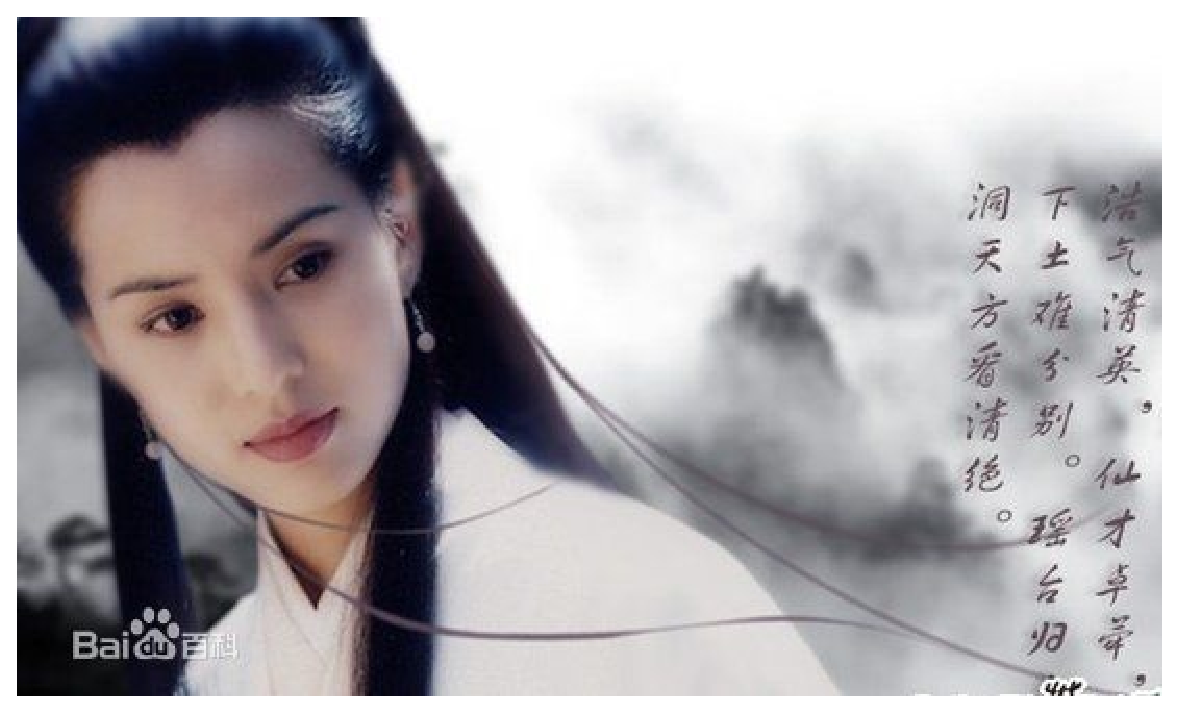
\includegraphics[width=\textwidth]{lrt}
  \caption{香中别有韵,清极不知寒}
  \label{fig:lrt}    
\end{figure}

图\ref{fig:lrt}是一个插图的例子。

图\ref{fig:lrt2}是另一个插图的例子。

\begin{figure}[!htbp]
  \centering
  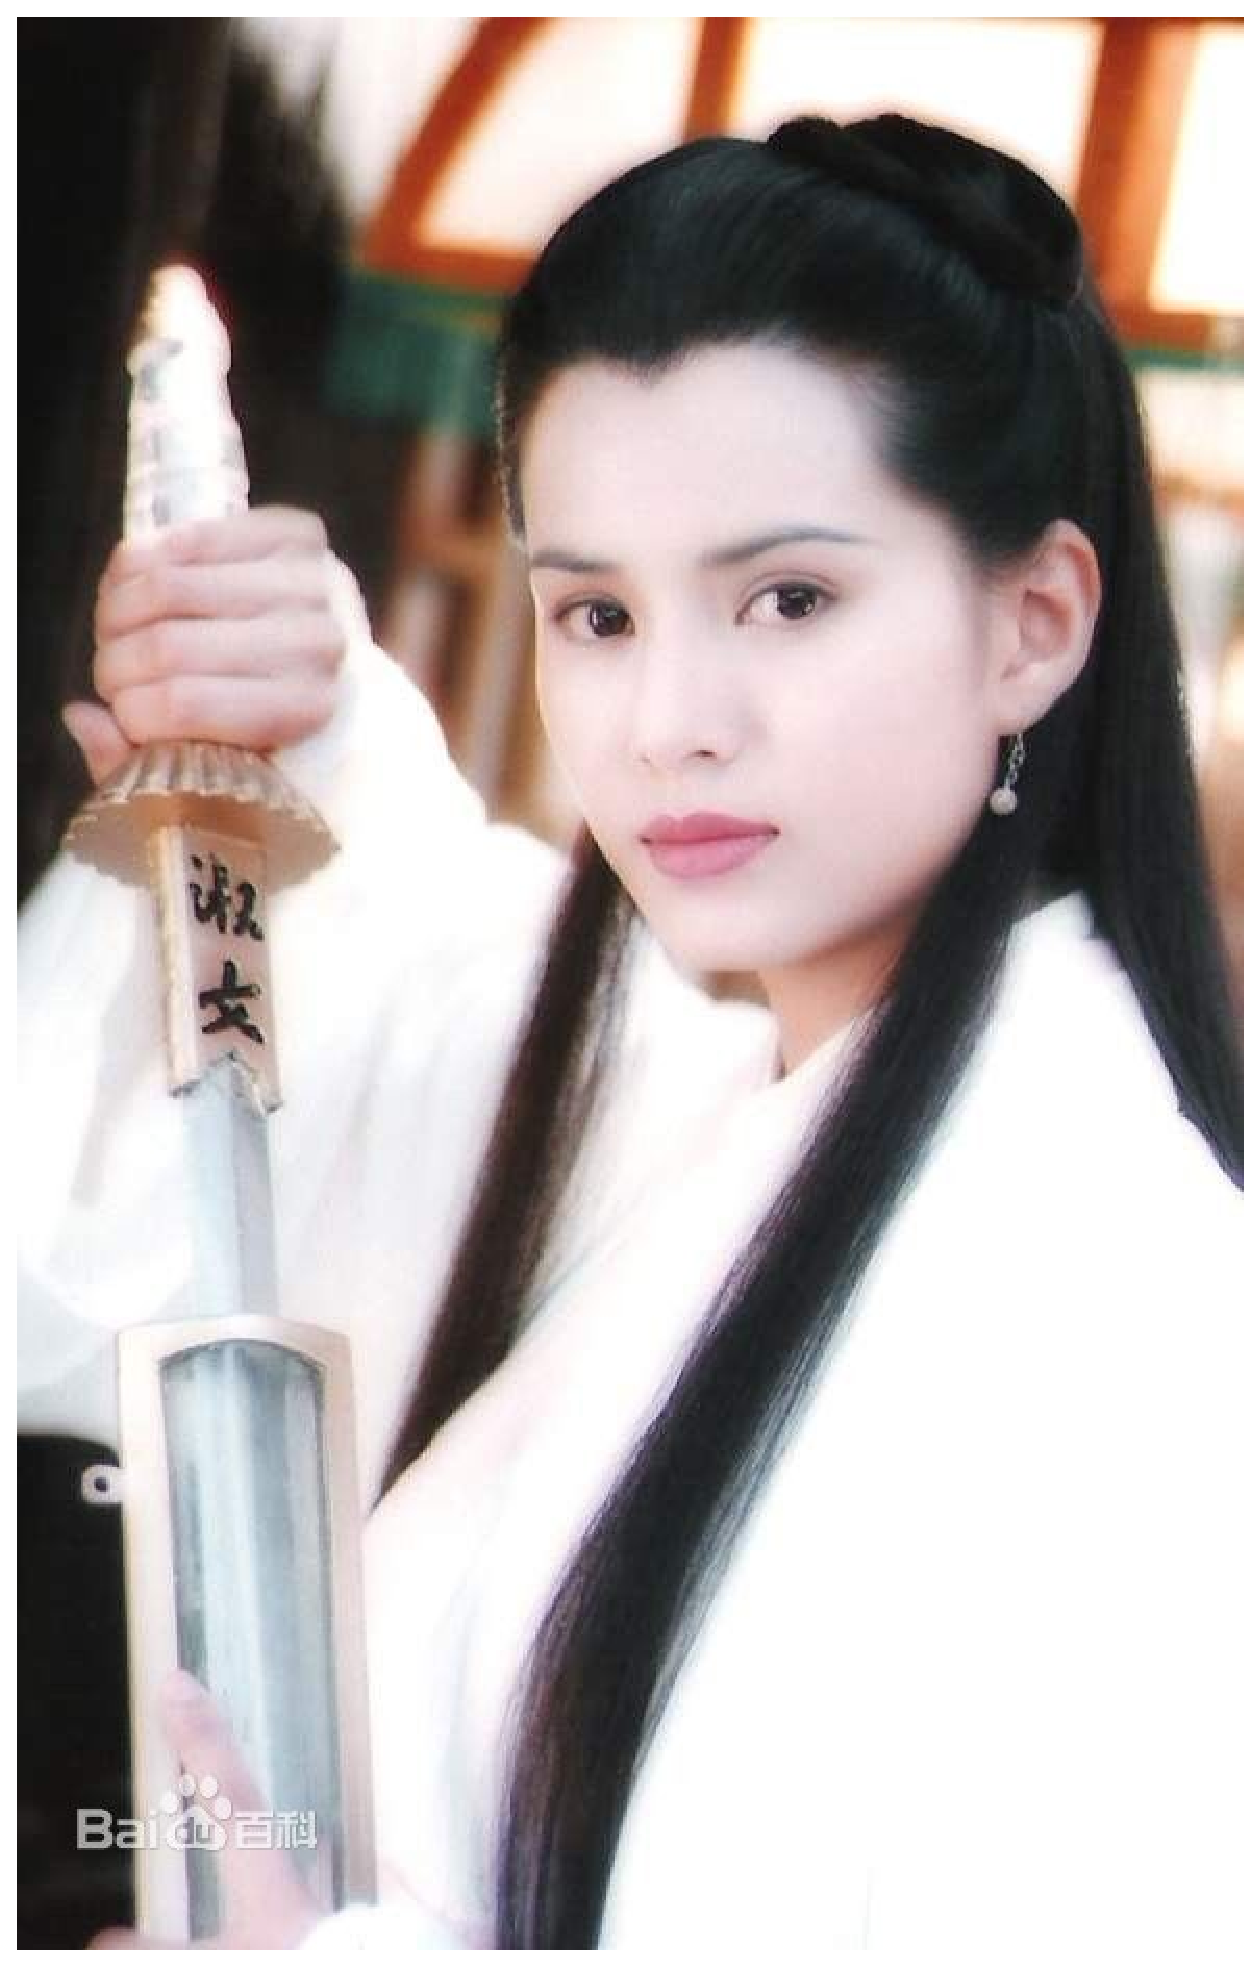
\includegraphics[height=3.5in]{lrt2}
  \caption{翩若游龙,宛若惊鸿}
  \label{fig:lrt2}    
\end{figure}


\section{表格}
\esection{Table}

\begin{table}[htbp]
  \centering
  \caption{这是一个自动编号的表格例子}
  \label{tab:tbl}
  \begin{tabular}[c]{|c|m{0.8in}|c|c|c|c|c|}\hline
    \multicolumn{2}{|c|}{Network Topology} & \# of nodes & 
    \multicolumn{3}{c|}{\# of clients} & Server \\\hline
    GT-ITM & Waxman Transit-Stub & 600 &
    \multirow{2}{2em}{2\%}& 
    \multirow{2}{2em}{10\%}& 
    \multirow{2}{2em}{50\%}& 
    \multirow{2}{1.2in}{Max. Connectivity}\\\cline{1-3}
    \multicolumn{2}{|c|}{Inet-2.1} & 6000 & & & &\\\hline
    \multirow{2}{1in}{blabla} & ban  & ban &\multicolumn{4}{c|}{\multirow{2}*{\sduthesis}}\\\cline{2-3}
    & \multicolumn{2}{c|}{ABCDEF} &\multicolumn{4}{c|}{} \\\hline
\end{tabular}  
\end{table}


\section{公式}
\esection{Equation}

首先,有行内公式,如$H~:~\mathcal{C}_n \rightarrow \mathcal{D}_n = \{0,1\}^\lambda$。

然后,有独立成行的不带编号的公式,如
$$
\forall\mathbf{y}\in\Lambda,\quad\mathcal{D}_{\Lambda,s,\mathbf{c}}(\mathbf{y})=\frac{\rho_{s,\mathbf{c}}(\mathbf{y})}{\rho_{s,\mathbf{c}}(\Lambda)}
$$

接下来,就是正常的带编号的公式了,如
\begin{equation}
  \mathbf{Adv}^{eu\mbox{-}acma}_{\Pi}(\mathcal{A}) =  \Pr \left[\mathsf{Sig}\mbox{-}forge_{\mathcal{A},\Pi}(n) = 1 \right] \leq \mathsf{negl}(n).
\end{equation}


\section{算法}
\esection{Algorithm}

\begin{algorithm}
  \caption{算法名称}
\label{alg:alg}
  \algorithmicrequire 输入参数 \\
  \algorithmicensure 输出结果
  \begin{enumerate}
    \item 步骤1
    \item 步骤2
    \item 步骤3
  \end{enumerate}
\end{algorithm}


\section{定义}
\esection{Definition}

\begin{definition}[格]
\label{def:lattice}
给定一组线性无关的向量$\mathbf{B}=\left\{\mathbf{b}_1,\cdots,\mathbf{b}_n\right\}\in\mathbb{R}^{m\times n}$,定义
\begin{equation}
\mathcal{L}(\mathbf{B})=\mathcal{L}(\mathbf{b}_1,\cdots,\mathbf{b}_n)=\left\{\sum_{i\in[n]}x_i\mathbf{b}_i\mid x_i\in\mathbb{Z}\right\}
\end{equation}
为$\mathbf{B}$上的格。其中,线性无关向量组$\mathbf{B}$称作格的\textit{基},$m$和$n$分别称作格的\textit{维}和\textit{秩}。
\end{definition}

定义\ref{def:lattice}是一个定义的例子。


\section{定理}
\esection{Theorem}

\begin{lemma}
\label{lem:basis}
      $\{\mathbf{b}_1,\cdots,\mathbf{b}_n\}$是(有序)基,另一有序基$\{\mathbf{d}_n,\cdots,\mathbf{d}_1\}$是前者对偶基的逆序,那么$\tilde{\mathbf{d}_i}=\tilde{\mathbf{b}_i}/\lVert\tilde{\mathbf{b}_i}\rVert^2(i\in[n])$。
\end{lemma}

引理\ref{lem:basis}是一个引理的例子。其它定理环境参见 sduthesis.pdf 3.6节数学环境。


\section{证明}
\esection{Proof}

\begin{proof}
这是一个证明环境,证明结束的地方会显示一个小黑块。
\end{proof}


\section{其它}
\esection{Others}

不带编号列表:

\begin{itemize}
  \item 无编号
  \item 每项前面有小圆点
  \item 可嵌套
  \begin{itemize}
    \item 最多嵌套3层
    \begin{itemize}
      \item 最多嵌套3层
      \begin{itemize}
        \item 最多嵌套3层
      \end{itemize}
    \end{itemize}
  \end{itemize}
  \item 无编号
\end{itemize}

编号列表:

\begin{enumerate}
  \item 有编号
  \item 可嵌套
  \begin{enumerate}
    \item 第1层嵌套
    \item 最多嵌套3层
    \begin{enumerate}
      \item 最多嵌套3层
        \begin{enumerate}
          \item 最多嵌套3层
        \end{enumerate}
    \end{enumerate}
  \end{enumerate}
  \item 这是顶层条目
\end{enumerate}


%%%
%%% End of File
%%%



%%% 3.后续部分
\backmatter
% 附录
\begin{appendix}
%%% Local Variables: 
%%% mode: latex
%%% TeX-master: "../main"
%%% End: 

\chapter{特殊浮动对象}
\echapter{Special Float Object}
\label{cha:speobj}
如果附录中的公式不想让它出现在公式索引中,那就请用 \verb|\tag*{xxx}|

\begin{equation}\tag*{(123)} 
\left\{\begin{array}{l}
\max \,\,f(x)\\[0.1 cm]
\mbox{subject to:} \\ [0.1 cm]
\qquad g_j(x)\le 0,\quad j=1,2,\cdots,p
\end{array}\right.
\end{equation}

\begin{table}[ht]
  \centering
  \caption*{Table~111\hskip1em This is an example for manually numbered table, which
    would not appear in the list of tables}
  \label{tab:badtabular2}
  \begin{tabular}[c]{|c|m{0.8in}|c|c|c|c|c|}\hline
    \multicolumn{2}{|c|}{Network Topology} & \# of nodes & 
    \multicolumn{3}{c|}{\# of clients} & Server \\\hline
    GT-ITM & Waxman Transit-Stub & 600 &
    \multirow{2}{2em}{2\%}& 
    \multirow{2}{2em}{10\%}& 
    \multirow{2}{2em}{50\%}& 
    \multirow{2}{1.2in}{Max. Connectivity}\\\cline{1-3}
    \multicolumn{2}{|c|}{Inet-2.1} & 6000 & & & &\\\hline
    \multirow{2}{1in}{blahblah} & jin  & jin &\multicolumn{4}{c|}{\multirow{2}*{\sduthesis}}\\\cline{2-3}
    & \multicolumn{2}{c|}{ABCDEF} &\multicolumn{4}{c|}{} \\\hline
\end{tabular}  
\end{table}

\begin{figure}[h]
  \centering
  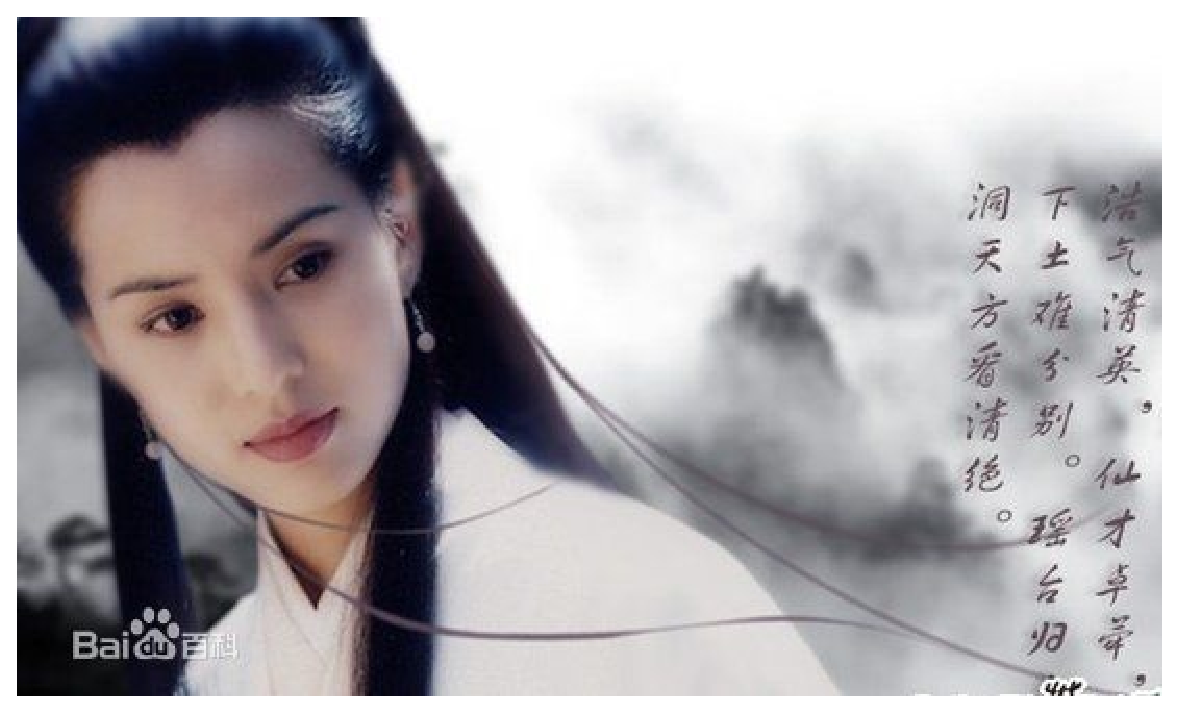
\includegraphics[width=\textwidth]{lrt}
  \caption*{Figure~123\hskip1em This is an example for manually numbered figure,
    which would not appear in the list of figures}
  \label{tab:badfigure2}    
\end{figure}

\begin{table}[ht]
\centering
  \centering
  \caption*{表~222\hskip1em 这是手动编号但不出现在索引中的表格例子}
  \label{tab:badtabular3}
  \begin{tabular}[c]{|c|m{0.8in}|c|c|c|c|c|}\hline
    \multicolumn{2}{|c|}{Network Topology} & \# of nodes & 
    \multicolumn{3}{c|}{\# of clients} & Server \\\hline
    GT-ITM & Waxman Transit-Stub & 600 &
    \multirow{2}{2em}{2\%}& 
    \multirow{2}{2em}{10\%}& 
    \multirow{2}{2em}{50\%}& 
    \multirow{2}{1.2in}{Max. Connectivity}\\\cline{1-3}
    \multicolumn{2}{|c|}{Inet-2.1} & 6000 & & & &\\\hline
    \multirow{2}{1in}{blah} & blah  & jin &\multicolumn{4}{c|}{\multirow{2}*{\sduthesis}}\\\cline{2-3}
    & \multicolumn{2}{c|}{ABCDEF} &\multicolumn{4}{c|}{} \\\hline
\end{tabular}  
\end{table}

\begin{figure}[!htbp]
  \centering
  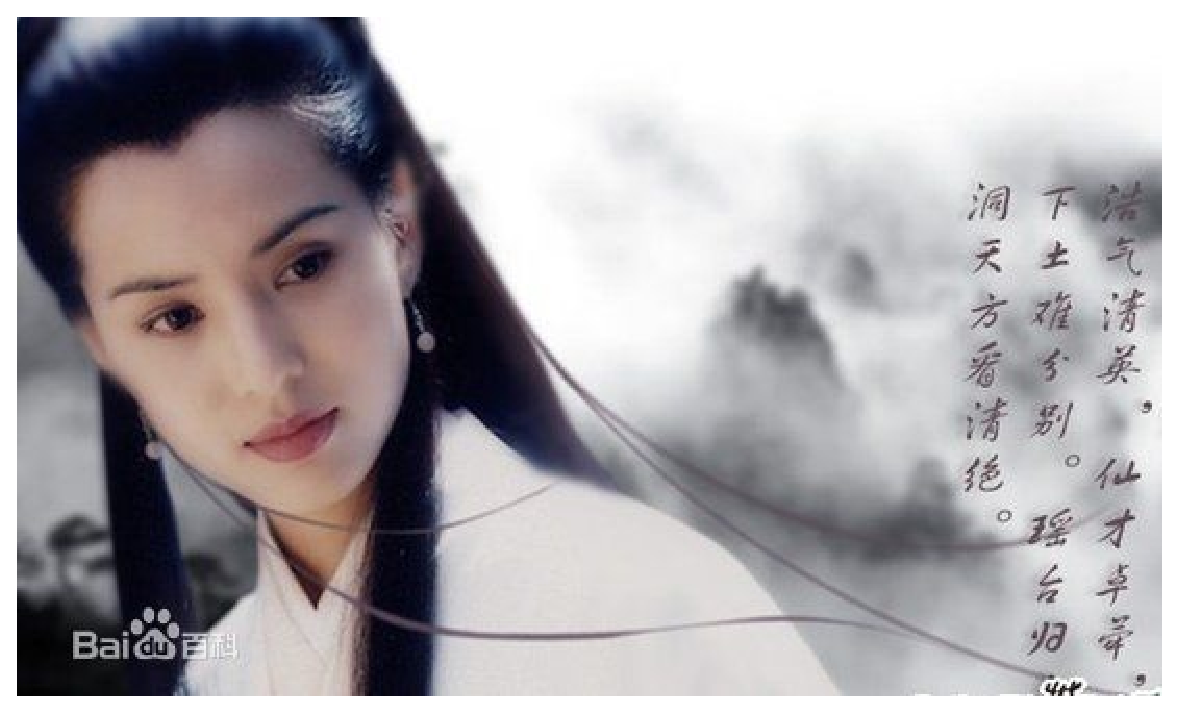
\includegraphics[width=\textwidth]{lrt}
  \caption*{图~321\hskip1em 这是手动编号但不出现索引中的图片例子}
  \label{tab:badfigure3}    
\end{figure}

%%%
%%% End of File
%%%

\chapter{逍遥游}
\echapter{Xiao Yao You}

北冥(míng)有鱼,其名为鲲(kūn)。鲲之大,不知其几千里也。化而为鸟,其名为鹏。鹏之背,不知其几千里也;怒而飞,其翼若垂天之云。是鸟也,海运则将徙(xǐ)于南冥。南冥者,天
池也。齐谐者,志怪者也。谐之言曰:“鹏之徙于南冥也,水击三千里,抟(tuán)扶摇而上者九万里,去以六月息者也。”野马也,尘埃也,生物之以息相吹也。天之苍苍,其正色邪(yé)?其远
而无所至极邪?其视下也,亦若是则已矣。且夫水之积也不厚,则其负大舟也无力。覆杯水于坳(ào)堂之上,则芥(jiè)为之舟,置杯焉则胶,水浅而舟大也。风之积也不厚,则其负大翼也
无力。故九万里,则风斯在下矣,而后乃今培风;背负青天,而莫之夭阏(yāo è)者,而后乃今将图南。蜩(tiáo)与学鸠笑之曰:“我决(xuè)起而飞,抢(qiāng)榆枋(fāng),时则不至,
而控于地而已矣,奚以之九万里而南为?”适莽(mǎng)苍者,三餐而反,腹犹果然;适百里者,宿(xiu)舂(chōng)粮;适千里者,三月聚粮。之二虫又何知!

小知(zhì)不及大知(32),小年不及大年。奚以知其然也?朝(zhāo)菌(jūn)不知晦朔(huì shuò),蟪蛄不知春秋,此小年也。楚之南有冥灵者,以五百岁为春,五百岁为秋;上古有大椿
(chūn)者,以八千岁为春,八千岁为秋,此大年也。而彭祖乃今以久特闻,众人匹之,不亦悲乎!汤之问棘也是已。(汤问棘曰:‘上下四方有极乎?’棘曰:'无极之外复无极也。【注】)穷发
(fà)之北,有冥海者,天池也。有鱼焉,其广数千里,未有知其修者,其名为鲲。有鸟焉,其名为鹏,背若泰山,翼若垂天之云,抟扶摇羊角而上者九万里,绝云气,负青天,然后图南,且适
南冥也。斥鴳(yàn)笑之曰:‘彼且奚适也?我腾跃而上,不过数仞而下,翱翔蓬蒿之间,此亦飞之至也。而彼且奚适也?’”此小大之辩也。

故夫知(zhì)效一官,行比一乡,德合一君,而(néng)征一国者,其自视也亦若此矣。而宋荣子犹然笑之。且举世而誉之而不加劝,举世而非之而不加沮(jǔ),定乎内外之分,辩乎荣辱之境,
斯已矣。彼其于世,未数(shuò)数(shuò)然也。虽然,犹有未树也。夫列子御风而行,泠(líng)然善也,旬有(yòu)五日而后反。彼于致福者,未数数然也。此虽免乎行,犹有所待者也。
若夫乘天地之正,而御六气之辩,以游无穷者,彼且恶乎待哉?故曰:至人无己,神人无功,圣人无名。


\end{appendix}

% 参考文献
\bibliographystyle{sdubib}
\bibliography{ref/kungfu}

% 致谢
%%% Local Variables:
%%% mode: latex
%%% TeX-master: "../main"
%%% End:

\chapter{致\hspace{1em}谢}
\echapter{Acknowledgement}

在这里写一些感谢的话。

感谢导师,感谢学科组老师,感谢师兄弟、师姐妹,感谢朋友和家人等等等等等。

感谢学校,感谢社会,感谢教育,感谢国家。好吧。

感谢 \sduthesis{},为我的论文排版节约了大量时间。

感谢王伊蕾师姐提供的学位论文评阅及答辩情况表格代码,和外文论文排版代码,以及对博士论文格式的悉心校对。

%%%
%%% End of File
%%%


% 攻读学位期间发表的学术论文/参与的科研项目
\chapter{攻读硕士学位期间完成论文情况}
\echapter{Paper Published}

\begin{enumerate}
    \item \textbf{Guo Jing} and Huang Yaoshi. ``桃花岛花草养殖综述.'' 桃花岛学报, 1250 9th International Conference on. MISC, 1250.
    \item \textbf{Guo Jing} and Hong Qigong. ``降龙十八掌掌法精要.'' 武林学报, 1245 12th International Conference on. KungFu, 1245.
\end{enumerate}


\chapter{攻读学位期间参与科研项目情况}
\echapter{Research Projects Participated}

\begin{enumerate}
    \item 桃花岛导弹防御系统的研究与开发~~桃花岛973项目(No.1244THD10188)
\end{enumerate}


% 学位论文评阅及答辩情况表
\makeevaluation

% 表格、插图、公式索引。带*的版本不生成目录项
% 山东大学没有索引的要求,Just in case.
%\listoftables
%\listoffigures
%\listofequations*

\end{document}
%%%
%%% End of 'main.tex'
%%%
